% Part of the team paper; included by main.tex (and by nathan_sections.tex for the standalone preview).
% ============================================================================================
\section{Results}
\label{sec:results}

\subsection{The transformer learns to use its context}
Figure~\ref{fig:training} shows training. With correct-goal demonstrations, validation error at $k = 4$ falls from 0.015 to 0.0015,
while error with wrong-goal demonstrations \emph{rises} from 0.020 to 0.14 over the same steps. The model becomes more committed to
the goal its context implies, even when that goal is wrong. Without demonstrations the error levels off at 0.0044, about $3\times$ the
correct-goal error; this is the error this model reaches without the goal, not a proven lower bound. The checkpoint with the lowest validation error was the final one
(step 100k), and validation error was still falling slowly, so longer training might help.

\begin{figure}[h]
  \centering
  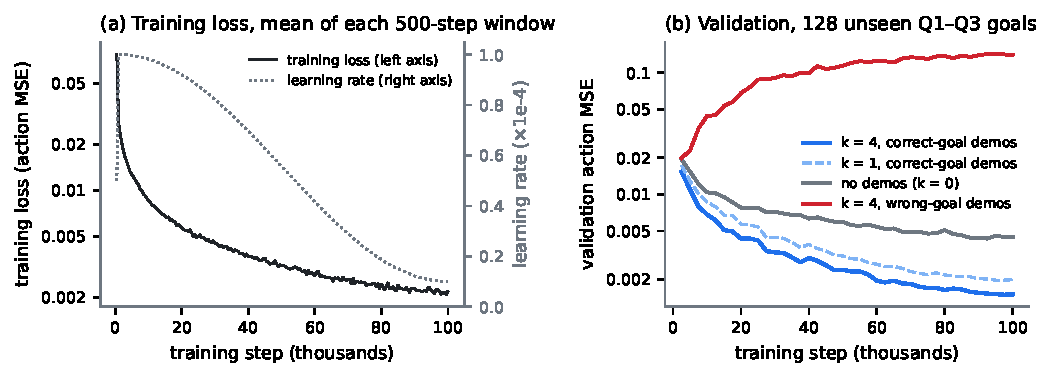
\includegraphics[width=\linewidth]{figures/fig_training.pdf}
  \caption{\textbf{Training.} (a) Training loss, the mean of each 500-step window over prompts of all $k$ (solid, left axis), and
  the learning-rate schedule (dotted, right axis). (b) Validation action MSE on 128 unseen $Q_1$--$Q_3$ goals, every 2{,}500 steps.
  Both loss axes are logarithmic because the errors span two orders of magnitude. What to notice: as the correct-goal error falls,
  the wrong-goal error \emph{rises}, so the model relies more and more on its context.}
  \label{fig:training}
\end{figure}

\subsection{In distribution, in-context control matches the teachers}
Table~\ref{tab:main} gives closed-loop success at $k = 4$. On unseen $Q_1$--$Q_3$ goals, the transformer reaches 91.2\% / 87.5\%
success-once / at-end with PPO demonstrations and 91.6\% / 87.5\% with BC demonstrations. That is within the confidence intervals
of the teachers that see the goal (94.1\% / 89.1\% and 92.0\% / 85.9\%). Under the controls it collapses: 1.4--1.6\% success-once
with wrong-goal demonstrations and 0.8--1.4\% with none. Every condition runs from the same initial states, so the gap of about
90 points is caused by the content of the context alone.

\begin{table}[h]
\centering
\caption{\textbf{Closed-loop success at $k = 4$} (\%; 512 episodes per cell, 95\% Wilson interval in brackets). One checkpoint throughout;
``Prompt'' names the teacher that recorded the demonstrations in its prompt. All conditions in a row use the same initial states.}
\label{tab:main}
\small
\begin{tabular}{lllcccc}
\toprule
Goals & Prompt & Metric & Correct goal & Wrong goal & No demos & Teacher (sees $g$) \\
\midrule
$Q_1$--$Q_3$ & PPO & once   & 91.2 [88.4, 93.4] & 1.4 [0.7, 2.8] & 1.4 [0.7, 2.8] & 94.1 [91.8, 95.9] \\
             &     & at end & 87.5 [84.4, 90.1] & 1.0 [0.4, 2.3] & 0.4 [0.1, 1.4] & 89.1 [86.1, 91.5] \\
             & BC  & once   & 91.6 [88.9, 93.7] & 1.6 [0.8, 3.1] & 0.8 [0.3, 2.0] & 92.0 [89.3, 94.0] \\
             &     & at end & 87.5 [84.4, 90.1] & 0.8 [0.3, 2.0] & 0.4 [0.1, 1.4] & 85.9 [82.7, 88.7] \\
\midrule
$Q_4$ (held out) & PPO & once   & 86.1 [82.9, 88.9] & 3.9 [2.5, 6.0] & 0.2 [0.0, 1.1] & 94.7 [92.4, 96.4] \\
                 &     & at end & 67.0 [62.8, 70.9] & 0.0 [0.0, 0.7] & 0.0 [0.0, 0.7] & 92.6 [90.0, 94.5] \\
                 & BC  & once   & 88.5 [85.4, 91.0] & 3.5 [2.2, 5.5] & 0.2 [0.0, 1.1] & 94.9 [92.7, 96.5] \\
                 &     & at end & 63.7 [59.4, 67.7] & 0.4 [0.1, 1.4] & 0.0 [0.0, 0.7] & 93.6 [91.1, 95.4] \\
\bottomrule
\end{tabular}
\end{table}

\textbf{PPO and BC prompts give the same results, by construction.} The same checkpoint, prompted with either teacher's
demonstrations, reaches the same success within the confidence intervals (Table~\ref{tab:main}, Figure~\ref{fig:k}). This says
little about generalizing across teacher types: in v1 the BC teacher is distilled from the PPO teacher, so the two produce nearly
identical demonstrations, starting from the same initial states and differing only by BC's small imitation error. We
intended PPO and BC to be distinct types of demonstrator. Testing that needs a BC teacher trained independently of PPO and a separate
learner per teacher type (Section~\ref{sec:conclusion}).

\subsection{One demonstration is nearly enough}
Figure~\ref{fig:k} varies $k$. A single demonstration already gives 90--91\% success-once on $Q_1$--$Q_3$, and $k \ge 2$ mainly
improves success-at-end (82--84\% at $k = 1$, 88\% at $k = 2$). Beyond $k = 2$ the curves are flat within their intervals. This fits
the task: the goal is a 2-D position, and one successful demonstration shows where the T ended up, which is almost the goal itself.
We return to this in Section~\ref{sec:conclusion}.
Teacher-forced error is slightly higher at $k = 8$ than at $k = 4$, which does not show in closed loop
(Appendix~\ref{app:action-error}).

\begin{figure}[h]
  \centering
  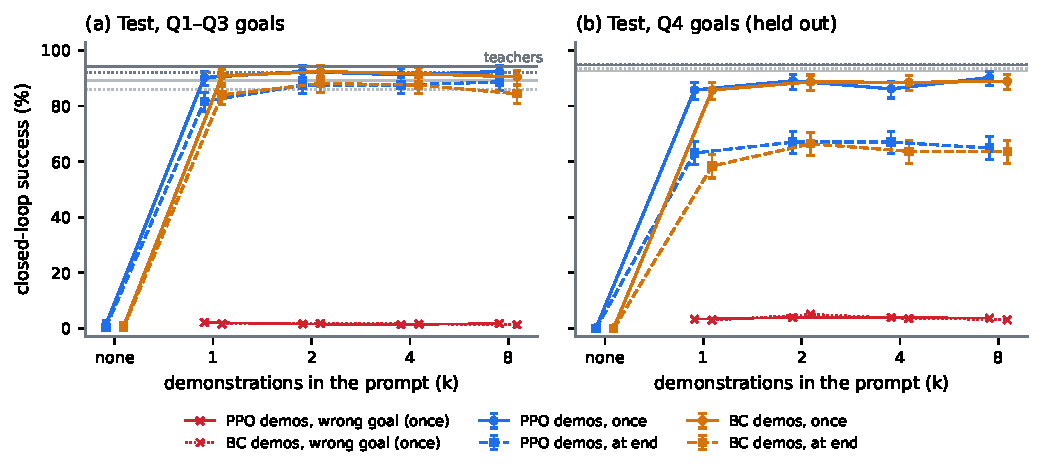
\includegraphics[width=\linewidth]{figures/fig_success_vs_k.pdf}
  \caption{\textbf{Closed-loop success vs number of demonstrations $k$} for unseen goals in $Q_1$--$Q_3$ (a) and held-out $Q_4$ goals
  (b). Colour gives the teacher that recorded the prompt (blue PPO, orange BC). Solid lines with circles show success-once and dashed
  lines with squares success-at-end, both with correct-goal demonstrations; crosses show success-once with wrong-goal demonstrations.
  The ``none'' point is the no-demonstration control. Grey lines mark the goal-seeing PPO teacher (BC teacher in Table~\ref{tab:main}).
  The $x$ axis is categorical. Error bars are 95\% Wilson intervals over 512 episodes (one training seed); PPO and BC points are offset
  slightly in $x$. What to notice: one demonstration is nearly enough, and on $Q_4$ success-at-end stays about 20--25 points below
  success-once.}
  \label{fig:k}
\end{figure}

\subsection{Held-out goals: reaching transfers, holding does not}
On $Q_4$ goals, which the transformer never trained on, the controls still behave as before: at most 3.9\% with wrong-goal
demonstrations and 0.2\% with none. The model reads held-out goals from its context. Success-once stays high (86.1--88.5\%, against
94.7--94.9\% for the teachers), but success-at-end drops to 63.7--67.0\% against the teachers' 92.6--93.6\%. In distribution, the
transformer loses about 4 points between success-once and success-at-end; on $Q_4$ it loses 19--25. This suggests that in roughly
a quarter of $Q_4$ episodes it brings the T onto the goal and then pushes it off again. We infer this from the two metrics and have
not yet inspected the trajectories. Extra demonstrations do not fix this: success-at-end
levels off at 64--67\% from $k = 2$ (Figure~\ref{fig:k}b). Teacher-forced error tells the same story: 0.0027 on $Q_4$ against 0.0016 in
distribution at $k = 4$. That is still 3$\times$ better than no context, but enough to matter for fine positioning. Our reading:
the coarse behavior, pushing toward the goal the context implies, generalizes to new goal positions. The precise corrective
actions near an unfamiliar goal do not.

\subsection{Offline error alone does not predict closed-loop success}
\label{sec:threshold}
A 3k-step pilot with the same settings reached validation action MSE 0.013 at $k = 4$, about $9\times$ the final model's, and already
preferred correct over wrong demonstrations (0.013 vs 0.016). In closed loop it scored 0\% under every condition, in a smaller
evaluation of 64 validation goals $\times$ 2 starts, while the teachers scored 91--94\% on the same starts. The final model, at
0.0015, matches the teachers. Two models are too few to locate a threshold. They do show that a model can prefer the right
demonstrations offline and still fail completely in closed loop, because small per-step errors compound over 100 steps, so
closed-loop evaluation is necessary.

\subsection{Comparison with an independent implementation}
\label{sec:compare}
One of the authors independently implemented and trained the same architecture with the same teachers, split sizes and closed-loop
protocol, in a separate codebase that collected its own demonstrations, for 50k steps at a constant learning rate in fp16 (two
seeds). Teacher success on the evaluation starts matches ours exactly, so the evaluation episodes are identical and the
closed-loop numbers are directly comparable (Table~\ref{tab:compare}). Both runs show the same qualitative results: success
comes from the context, about 0\% under both controls, $k = 1$ gives most of the effect, PPO and BC prompts give the same
results, and $Q_4$ success-at-end drops. Our run is stronger: success-once is 8 points higher and success-at-end 20 points
higher in distribution, consistent with its roughly $3\times$ lower action error.

\textbf{This comparison is not controlled.} Training length, learning-rate schedule, numeric precision and code all differ at once,
so we cannot attribute the gap to one of them. At 50k steps, the length of the independent run, our validation error was already 0.0024, below that run's
final 0.004--0.006. That suggests the decaying learning rate matters, not only the extra steps. A one-factor test is to rerun the
independent code with our schedule. Its two seeds also differ by 31 points in $Q_4$ success-at-end (41\% vs 72\%, PPO demos, $k = 4$), while
success-once is stable (77\% vs 79\%). Our single-seed $Q_4$ success-at-end therefore has wide uncertainty beyond the binomial
interval in Table~\ref{tab:main}. Success-once and the in-distribution results look stable.

